\section{Rappel sur les opérateurs vectoriels --- Et pour aller plus loin}
This last chapter does three unrelated jobs. It first collects, as a
reference sheet, les opérateurs différentiels mathématiques appliqués dans un
repère de coordonnées cartésiennes, with which every propagation equation of the
course is written. It then lifts the perfect MLHI hypothesis of Chapter 2 and
lets the medium have losses --- a \textit{diélectrique imparfait} on one side, a
\textit{conducteur imparfait} on the other --- and reads off what the loss does
to the vecteur d'onde and to the fields. It closes by opening onto an area of
current research: the métamatériaux, artificial structures whose permittivité
effective and perméabilité effective take values no natural material offers,
including negative ones.

\begin{notation}
  The operators have a French-style notation,
  $\overrightarrow{\mathrm{grad}}$, $\mathrm{div}$,
  $\overrightarrow{\mathrm{rot}}$, $\Delta$; these notes write $\grad$, $\div$,
  $\curl$ and $\Delta$ for the same four. The cross product is $\wedge$
  throughout, so $\curl\v{F}$ and $\grad\wedge\v{F}$ denote
  the same vector. Vectors are bold: $\v{E}$, $\v{H}$, $\v{F}$, $\v{k}$.\\

  Two collisions of symbols are worth fixing before anything else.
  \begin{subpart}
    \item The \emph{scalar} field of the gradient is written
      $F_{x,y,z}$, meaning $F(x,y,z)$ --- not a component. The components of a
      \emph{vector} field are $F_x$, $F_y$, $F_z$ with a single subscript.
    \item In this chapter $\delta$ is the épaisseur de peau. In Chapter 2 the
      same letter is the angle de perte of the complex permittivité. They are
      different quantities.
  \end{subpart}
  As everywhere in the course the time convention is $e^{+j\omega t}$, so a
  wave travelling towards increasing $z$ carries $e^{j(\omega t - k_z z)}$ and
  the phase spatiale enters with a minus sign.
\end{notation}

\subsection{Définition des opérateurs différentiels utilisés pour la résolution des équations de propagation d'ondes électromagnétiques en coordonnées cartésiennes}

Everything below is stated for a vector field. Soit un vecteur $\v{F}(x,y,z)$
dépendant des variables d'espace définies dans le repère $(O,X,Y,Z)$ :
\[
  \v{F}(x,y,z) = F_x\,\unitv{u}_x + F_y\,\unitv{u}_y + F_z\,\unitv{u}_z ,
\]
où $F_x$, $F_y$, $F_z$ sont les composantes de $\v{F}$ et
$\unitv{u}_x,\unitv{u}_y,\unitv{u}_z$ représentent le système de vecteurs
unitaires associé au repère.
This section is a reference sheet, not a derivation: the six results are used
without further comment in Chapters 2 and 3.

\begin{center}
  \begin{tabular}{llll}
    \toprule
    Operator & French notation & $\grad$ form & Acts on $\to$ gives \\
    \midrule
    nabla & $\vec{\nabla}$ & $\grad$ & --- \\
    gradient & $\overrightarrow{\mathrm{grad}}\,(F_{x,y,z})$ & $\grad F$
      & scalar $\to$ vector \\
    divergence & $\mathrm{div}(\v{F})$ & $\div\v{F}$
      & vector $\to$ scalar \\
    rotationnel & $\overrightarrow{\mathrm{rot}}\,(\v{F})$
      & $\grad\wedge\v{F}$ & vector $\to$ vector \\
    scalar Laplacian & $\Delta(F_x)$ & $\div\grad F_x$
      & scalar $\to$ scalar \\
    vector Laplacian & $\Delta(\v{F})$ & $\grad\cdot\grad\v{F}$
      & vector $\to$ vector \\
    \bottomrule
  \end{tabular}
\end{center}

\paragraph{Nabla.}
C'est l'opérateur différentiel générique qui sert à calculer le gradient, la
divergence, le rotationnel et le Laplacien. It expresses the variation (the
derivative) of a field as a function of its position in space:
\[
  \grad =
  \begin{pmatrix}
    \del/\del x \\[2pt] \del/\del y \\[2pt] \del/\del z
  \end{pmatrix}.
  \tag*{(1)}
\]

\paragraph{Gradient.}
En analyse vectorielle, le gradient est une grandeur \emph{vectorielle}
indiquant la variation d'une grandeur physique dans l'espace. On écrit :
\[
  \overrightarrow{\mathrm{grad}}\,(F_{x,y,z}) =
  \begin{pmatrix}
    \del F_{x,y,z}/\del x \\[2pt]
    \del F_{x,y,z}/\del y \\[2pt]
    \del F_{x,y,z}/\del z
  \end{pmatrix}
  = \grad F_{x,y,z}.
  \tag*{(2)}
\]
Il représente la variation de la valeur du champ \emph{scalaire} dans l'espace.
Colour gradients picture it: a concentric one, whose gradient arrows all point
at the centre, and a unidirectional one, whose arrows are parallel.

\paragraph{Divergence.}
D'une manière générale, la divergence est reliée en physique à l'expression
locale de la propriété de \emph{conservation} d'une grandeur. It turns a vector
field into a scalar; on écrit l'opérateur divergence de cette manière :
\[
  \mathrm{div}(\v{F}) = \frac{\del F_x}{\del x} + \frac{\del F_y}{\del y}
    + \frac{\del F_z}{\del z}.
  \tag*{(3)}
\]

\begin{remark}[Why the MLHI hypothesis saves work]
  Dans le cas d'un MLHI, le milieu est conservateur, dans ce cas
  \[ \div\v{F} = 0 . \]
  Cette propriété permet de simplifier la détermination de l'équation de
  propagation d'une onde électromagnétique dans un MLHI (chapitre 2): it kills
  the $\overrightarrow{\mathrm{grad}}\,(\mathrm{div}(\v{F}))$ term of the
  identity below and leaves a pure Laplacian.
\end{remark}

\paragraph{Rotationnel.}
L'opérateur rotationnel exprime la tendance qu'ont les lignes de champ d'un
champ vectoriel à tourner autour d'un point : sa circulation locale sur un
contour entourant ce point est non nulle quand son rotationnel ne l'est pas.
Par exemple : dans une tornade, le vent tourne autour de l'œil du cyclone et le
champ vectoriel vitesse du vent a un rotationnel non nul autour de l'œil du
cyclone. On développe le calcul ainsi :
\[
  \overrightarrow{\mathrm{rot}}\,(\v{F}) =
  \begin{pmatrix}
    \del F_z/\del y - \del F_y/\del z \\[2pt]
    \del F_x/\del z - \del F_z/\del x \\[2pt]
    \del F_y/\del x - \del F_x/\del y
  \end{pmatrix}
  = \grad \wedge \v{F}
  =
  \begin{pmatrix}
    \del/\del x \\[2pt] \del/\del y \\[2pt] \del/\del z
  \end{pmatrix}
  \wedge
  \begin{pmatrix} F_x \\ F_y \\ F_z \end{pmatrix}.
  \tag*{(4)}
\]
Le rotationnel de $\v{F}$ revient donc à faire le produit vectoriel de
$\grad$ avec $\v{F}$.

\begin{figure}[h!]
  \centering
  \begin{tikzpicture}[>=latex,scale=0.92]
    \draw[gray!50] (0,0) rectangle (3,3);
    \foreach \x in {0.45,1.05,1.65,2.25,2.85}
      \foreach \y in {0.45,1.05,1.65,2.25,2.85}
        \draw[->,thick] (\x-0.20,\y-0.20) -- (\x+0.20,\y+0.20);
    \node at (1.5,-0.5) {a. $\curl\v{F} = \v{0}$};
    \begin{scope}[xshift=4.6cm]
      \draw[gray!50] (0,0) rectangle (3,3);
      \foreach \r in {0.55,1.00,1.35}
        \foreach \t [evaluate=\t as \te using \t+34] in {0,45,...,315}
          \draw[->,thick] ([shift={(\t:\r)}]1.5,1.5)
             -- ([shift={(\te:\r)}]1.5,1.5);
      \node at (1.5,-0.5) {b. $\curl\v{F} \neq \v{0}$};
    \end{scope}
  \end{tikzpicture}
  \caption*{\small Exemple d'interprétation d'un rotationnel appliqué au
  vecteur $\v{F}$. A uniform field circulates to zero on every closed contour;
  a vortex does not.}
\end{figure}

\paragraph{Laplacien vectoriel.}
Le Laplacien vectoriel permet d'estimer la différence entre la valeur de
$\v{F}$ en un point quelconque du milieu et la valeur moyenne de $\v{F}$ au
voisinage de ce point. Component by component, on le définit par :
\[
  \Delta(\v{F}) = \grad\cdot\grad\v{F} =
  \begin{pmatrix}
    \del^2 F_x/\del x^2 + \del^2 F_x/\del y^2 + \del^2 F_x/\del z^2 \\[2pt]
    \del^2 F_y/\del x^2 + \del^2 F_y/\del y^2 + \del^2 F_y/\del z^2 \\[2pt]
    \del^2 F_z/\del x^2 + \del^2 F_z/\del y^2 + \del^2 F_z/\del z^2
  \end{pmatrix}
  =
  \begin{pmatrix} \Delta(F_x) \\ \Delta(F_y) \\ \Delta(F_z) \end{pmatrix}
  =
  \begin{pmatrix}
    \mathrm{div}\big(\overrightarrow{\mathrm{grad}}\,(F_x)\big) \\[2pt]
    \mathrm{div}\big(\overrightarrow{\mathrm{grad}}\,(F_y)\big) \\[2pt]
    \mathrm{div}\big(\overrightarrow{\mathrm{grad}}\,(F_z)\big)
  \end{pmatrix}.
  \tag*{(5)}
\]
The last equality is the definition of the \emph{scalar} Laplacian, which
enters here only implicitly, as $\Delta(F_x) = \mathrm{div}(\overrightarrow{\mathrm{grad}}\,(F_x))$
acting on each cartesian component separately.

\begin{theorem}[Relation fondamentale avec le Laplacien vectoriel]
  \[
    \overrightarrow{\mathrm{rot}}\Big(\overrightarrow{\mathrm{rot}}\,(\v{F})\Big)
    = \overrightarrow{\mathrm{grad}}\Big(\mathrm{div}(\v{F})\Big) - \Delta(\v{F}),
    \qquad\text{i.e.}\qquad
    \curl(\curl\v{F}) = \grad(\div\v{F}) - \Delta(\v{F}).
    \tag*{(6)}
  \]
\end{theorem}

Cette relation est importante pour résoudre les équations de Maxwell: it is
the one result of the section that is used rather than quoted. Taking
the curl of the Maxwell--Faraday equation and substituting Maxwell--Ampère
produces $\curl(\curl\v{E})$; the identity converts it into
$\grad(\div\v{E}) - \Delta(\v{E})$, and in a source-free MLHI the first term
vanishes, leaving the propagation equation solved in Chapter 2.

\begin{remark}
  The simplification of these operators in the particular case of an onde
  plane monochromatique is not carried out in this chapter; it is done where
  it is needed, in Chapter 2, where the wave is taken as
  $e^{j(\omega t - k_z z)}$ so that $\del/\del z$ becomes multiplication by
  $-jk_z$ and the transverse derivatives vanish.
\end{remark}

\subsection{Milieux imparfaits}

Dans le chapitre 2, nous avons présenté le cas de milieux linéaires homogènes
isotropes \emph{parfaits}: a diélectrique of permittivité $\varepsilon$ with
zero conductivité, so that the current density $\v{j}$ in Maxwell--Ampère is
zero and the wave travels without loss. Un \textbf{milieu imparfait}
(\textit{imperfect medium}) présente des pertes. Both cases below --- the
diélectrique imparfait and the conducteur imparfait --- make a non-zero current
density $\v{j}$ appear in the medium; nous présentons ici la conséquence sur
l'expression des champs ainsi que du vecteur d'onde.

\begin{definition}[Les deux régimes]
  Write $\sigma$ for the conductivité of the medium and $\varepsilon$ for its
  permittivité. The medium is treated as
  \begin{subpart}
    \item a \textbf{diélectrique imparfait} (\textit{imperfect dielectric})
      when le diélectrique présente une conductivité $\sigma$ non nulle mais
      $\sigma \ll \omega\varepsilon$;
    \item a \textbf{conducteur imparfait} (\textit{imperfect conductor})
      when, à l'inverse du cas précédent, la conductivité
      $\sigma \gg \omega\varepsilon$.
  \end{subpart}
  The classification is therefore made on the dimensionless ratio
  $\sigma/(\omega\varepsilon)$, and it depends on frequency: the same material
  can be a conducteur at basse fréquence and a diélectrique at high frequency.
\end{definition}

\begin{remark}
  That ratio is the \textbf{tangente de pertes} (\textit{loss tangent})
  $\tan\delta = \varepsilon''/\varepsilon'$ introduced in Chapter 2. The
  derivation below never writes $\tan\delta$ and never names it; it works
  directly with the two inequalities. Remember that $\delta$ in this chapter is
  the épaisseur de peau instead.
\end{remark}

\subsubsection{Cas d'un diélectrique imparfait}

Le diélectrique présente une conductivité $\sigma$ non nulle mais $\sigma \ll
\omega\varepsilon$. L'équation de Maxwell--Ampère s'écrit alors :
\[
  \overrightarrow{\mathrm{rot}}\,\big(\v{H}(z,t)\big)
  = \sigma\v{E}(z,t) + \varepsilon\frac{\del \v{E}(z,t)}{\del t}
  = \sigma\v{E}(z,t) + j\omega\varepsilon\v{E}(z,t)
  = j\omega\varepsilon(\omega)\,\v{E}(z,t),
  \tag*{(7)}
\]
the whole point being that the conduction term and the displacement term can be
merged into a single \emph{complex, frequency-dependent} permittivité
\[
  \varepsilon(\omega) = \varepsilon\left(1 - j\frac{\sigma}{\omega\varepsilon}\right),
  \qquad \varepsilon = \varepsilon_0\varepsilon_r .
\]
The medium is then formally the diélectrique parfait of Chapter 2 with
$\varepsilon$ replaced by $\varepsilon(\omega)$, and all the loss is carried by
the imaginary part.\\

En remplaçant $\varepsilon$ par $\varepsilon(\omega)$, la norme du vecteur
d'onde $\|\v{k}\| = k_z$, pour une OPPM se propageant suivant l'axe $Oz$,
s'écrit :
\[
  k_z^{\,2} = \omega^2\mu_0\varepsilon\left(1 - j\frac{\sigma}{\omega\varepsilon}\right),
  \tag*{(8)}
\]
ce qui donne (since $\sigma \ll \omega\varepsilon$ permits a first-order
expansion of the square root) :
\[
  \boxed{\;k_z \approx \omega\sqrt{\mu_0\varepsilon}
    \left(1 - j\frac{\sigma}{2\omega\varepsilon}\right).\;}
  \tag*{(9)}
\]

Sur l'axe $Oz$, les champs s'écrivent :
\[
  \begin{aligned}
    \v{E}(z,t) &= \v{E}_+(z)\;
      e^{-\sqrt{\mu_0/\varepsilon}\,(\sigma/2)\,z}\;
      e^{\,j(\omega t - \omega\sqrt{\mu_0\varepsilon}\,z)}, \\[2pt]
    \v{H}(z,t) &= \v{H}_+(z)\;
      e^{-\sqrt{\mu_0/\varepsilon}\,(\sigma/2)\,z}\;
      e^{\,j(\omega t - \omega\sqrt{\mu_0\varepsilon}\,z)}.
  \end{aligned}
  \tag*{(10, 11)}
\]

\begin{conclusion}
  Le terme
  $e^{-\sqrt{\mu_0/\varepsilon}\,(\sigma/2)\,z}$ --- a real exponential ---
  correspond à l'atténuation \emph{supplémentaire} de l'onde en fonction de
  $z$ par les pertes du milieu. Reading the two constants off the fields,
  \[
    \alpha = \frac{\sigma}{2}\sqrt{\frac{\mu_0}{\varepsilon}}
    \quad\text{(Np/m)},
    \qquad
    \beta = \omega\sqrt{\mu_0\varepsilon}
    \quad\text{(rad/m)} .
  \]
  To first order the constante de phase is exactly the lossless one of
  Chapter 2: a small conductivité attenuates the wave without changing its
  vitesse de phase.
\end{conclusion}

\subsubsection{Cas d'un conducteur imparfait}

À l'inverse du cas précédent, ici la conductivité $\sigma \gg \omega\varepsilon$:
the displacement term is negligible against the conduction term, and la norme
du vecteur d'onde sera donc égale à :
\[
  k_z^{\,2} \approx -j\omega\mu_0\sigma
  \tag*{(12)}
\]
soit
\[
  k_z \approx \pm\sqrt{\omega\mu_0\sigma}\,\sqrt{-j},
  \qquad \sqrt{-j} = \frac{j-1}{\sqrt{2}} ,
  \tag*{(13)}
\]
et $k_z$ devient :
\[
  k_z \approx \pm\sqrt{\omega\mu_0\sigma}\,\frac{j-1}{\sqrt{2}}
    = \pm\left(j\sqrt{\frac{\omega\mu_0\sigma}{2}} - \sqrt{\frac{\omega\mu_0\sigma}{2}}\right) .
  \tag*{(14)}
\]
Sur l'axe $Oz$, les champs s'écriront :
\[
  \begin{aligned}
    \v{E}(z,t) &= \v{E}_+(z)\;
      e^{-\sqrt{\omega\mu_0\sigma/2}\;z}\;
      e^{\,j\left(\omega t - \sqrt{\omega\mu_0\sigma/2}\;z\right)}, \\[2pt]
    \v{H}(z,t) &= \v{H}_+(z)\;
      e^{-\sqrt{\omega\mu_0\sigma/2}\;z}\;
      e^{\,j\left(\omega t - \sqrt{\omega\mu_0\sigma/2}\;z\right)} .
  \end{aligned}
  \tag*{(15, 16)}
\]

\begin{definition}[Épaisseur de peau (\textit{skin depth})]
  Le terme $\sqrt{\omega\mu_0\sigma/2}$ correspond à un \emph{effet
  pelliculaire}, ce qui indique la présence d'un courant simplement en
  périphérie et non au centre du conducteur. Il s'agit de la définition de la
  pénétration $\delta$ de l'onde dans le conducteur ou autrement appelé
  \textbf{effet de peau} (\textit{skin effect}) :
  \[
    \boxed{\;\delta = \sqrt{\frac{2}{\omega\mu_0\sigma}}\;}
  \]
  Plus la fréquence augmente plus l'épaisseur est fine.
\end{definition}

\begin{remark}[Sign bookkeeping in (14)]
  Both square roots of $-j$ are $\pm(1-j)/\sqrt{2}$, so the $\pm$ in front and
  the choice $\sqrt{-j} = (j-1)/\sqrt{2}$ together do cover the two roots. The
  root actually retained is the one that makes
  (15)--(16) decay towards increasing $z$, namely
  \[
    k_z = \sqrt{\frac{\omega\mu_0\sigma}{2}}\,(1 - j)
        = \frac{1}{\delta} - \frac{j}{\delta} .
  \]
  Read against $e^{j(\omega t - k_z z)}$ this gives $\alpha = \beta = 1/\delta$:
  in a good conducteur the constante d'atténuation and the constante de phase
  are equal. Two consequences worth remembering: the field amplitude falls by a
  factor $e$ over one épaisseur de peau, and the longueur d'onde inside the
  metal is $\lambda = 2\pi/\beta = 2\pi\delta$, so the wave is essentially
  extinguished within a fraction of one internal longueur d'onde.
\end{remark}

\begin{figure}[h!]
  \centering
  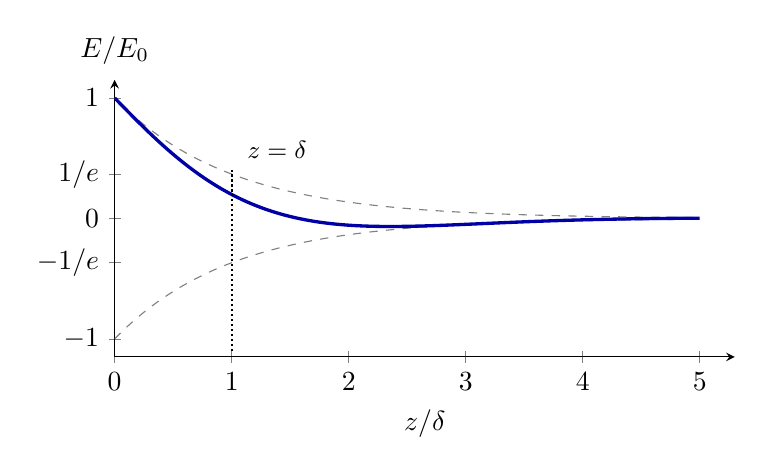
\begin{tikzpicture}
    \begin{axis}[
      width=0.78\textwidth, height=5.1cm,
      xlabel={$z/\delta$}, ylabel={$E/E_0$},
      axis lines=left, domain=0:5, samples=250,
      ymin=-1.15, ymax=1.15, xmin=0, xmax=5.3,
      xtick={0,1,2,3,4,5},
      ytick={-1,-0.368,0,0.368,1},
      yticklabels={$-1$,$-1/e$,$0$,$1/e$,$1$},
      every axis y label/.style={at={(ticklabel* cs:1.02)},anchor=south},
      ]
      \addplot[gray,dashed] {exp(-x)};
      \addplot[gray,dashed] {-exp(-x)};
      \addplot[blue!65!black,very thick] {exp(-x)*cos(deg(x))};
      \draw[densely dotted,thick] (axis cs:1,-1.1) -- (axis cs:1,0.40);
      \node[anchor=south west,font=\small] at (axis cs:1.05,0.42) {$z=\delta$};
    \end{axis}
  \end{tikzpicture}
  \caption*{\small Penetration of the field into a conducteur imparfait. With
  $\alpha = \beta = 1/\delta$ the envelope $e^{-z/\delta}$ and the oscillation
  $\cos(z/\delta)$ share the same scale: one épaisseur de peau costs a factor
  $1/e$ in amplitude and only one radian of phase.}
\end{figure}

\begin{example}[Where the transition sits --- the ground as a lossy medium]
  The ground is treated as a milieu non magnétique de permittivité
  complexe
  \[
    \bar{\epsilon} = \varepsilon - j\frac{\sigma}{\varepsilon_0\omega},
  \]
  and classified by a transition frequency: below $f_{\text{transition}}$
  it is a sol \emph{conducteur}, above it a sol \emph{diélectrique},
  with
  \[
    f_{\text{transition}} \sim 20~\text{GHz (pure water)},\quad
    \sim 1~\text{GHz (sea water)},\quad
    \sim 0.6\text{--}6~\text{MHz (non-maritime soils)} .
  \]
  The practical consequences are the prise en compte de l'image de l'antenne,
  and the correction du facteur de réflexion en fonction de la composition
  du sol, du relief et de la distance entre antennes.
\end{example}

\begin{remark}
  The ground's $\bar{\epsilon}$ and the diélectrique imparfait's
  $\varepsilon(\omega) = \varepsilon - j\sigma/\omega$ differ by a factor
  $\varepsilon_0$. They agree once the $\varepsilon$ of the ground is read as
  the \emph{relative} permittivité: then
  $\bar{\epsilon} = \varepsilon(\omega)/\varepsilon_0$. The criterion
  $\sigma/(\omega\varepsilon)$ is the same in both.
\end{remark}

\subsection{Métamatériaux}

\subsubsection{Introduction}

\begin{definition}[Métamatériau (\textit{metamaterial})]
  En physique, en électromagnétisme, le terme \textbf{métamatériau} sert à
  désigner un matériau \emph{artificiel} qui présente des propriétés
  électromagnétiques qu'on ne retrouve pas dans un matériau naturel. Il s'agit
  généralement de structures \emph{périodiques}, diélectriques ou métalliques,
  qui se comportent comme un matériau homogène n'existant pas à l'état naturel.
\end{definition}

Il existe plusieurs types de métamatériaux en électromagnétisme, les plus
connus étant ceux susceptibles de présenter à la fois une permittivité \emph{et}
une perméabilité négatives. Mais il en existe d'autres : milieux d'impédance
infinis, milieu à permittivité relative inférieure à $1$, etc. Materials are
classified on the quadrant plane $(\Re(\mu), \Re(\varepsilon))$.

\begin{figure}[h!]
  \centering
  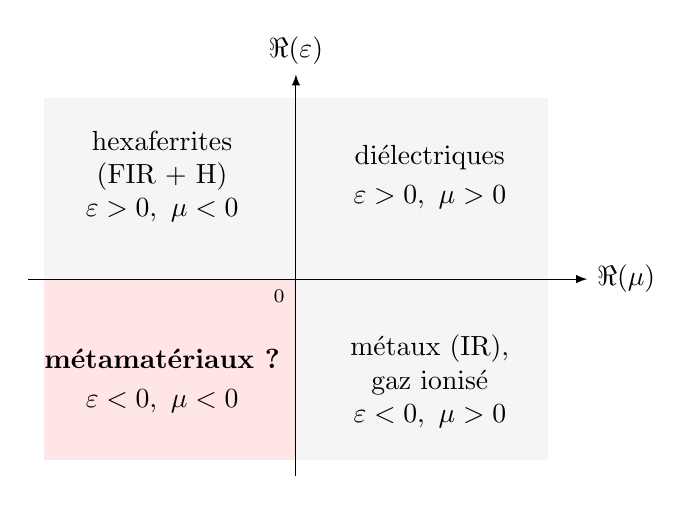
\begin{tikzpicture}[>=latex,scale=1.0]
    \fill[black!4] (-3.2,0) rectangle (3.2,2.3);
    \fill[black!4] (0,-2.3) rectangle (3.2,0);
    \fill[red!10] (-3.2,-2.3) rectangle (0,0);
    \draw[->] (-3.4,0) -- (3.7,0) node[right]{$\Re(\mu)$};
    \draw[->] (0,-2.5) -- (0,2.6) node[above]{$\Re(\varepsilon)$};
    \node[below left,font=\scriptsize] at (-0.02,-0.02) {$0$};
    \node[align=center] at (-1.7,1.3)
      {hexaferrites\\ (FIR + H)\\ $\varepsilon > 0,\ \mu < 0$};
    \node[align=center] at (1.7,1.3)
      {diélectriques\\[2pt] $\varepsilon > 0,\ \mu > 0$};
    \node[align=center] at (1.7,-1.3)
      {métaux (IR),\\ gaz ionisé\\ $\varepsilon < 0,\ \mu > 0$};
    \node[align=center] at (-1.7,-1.3)
      {\textbf{métamatériaux ?}\\[2pt] $\varepsilon < 0,\ \mu < 0$};
  \end{tikzpicture}
  \caption*{\small Classification des matériaux en fonction de leur
  permittivité $\varepsilon$ et perméabilité $\mu$. Three quadrants are
  populated by natural materials; the doubly negative one is the one that has
  to be built.}
\end{figure}

\begin{remark}[ENG and DNG]
  \textbf{ENG} (\textit{epsilon-negative}, $\varepsilon < 0$, $\mu > 0$) and
  \textbf{DNG} (\textit{double-negative}, $\varepsilon < 0$ \emph{and}
  $\mu < 0$) are the literature acronyms for two of the quadrants of the
  classification above, the second being the one labelled « métamatériaux ».
  They are not quadrant labels here --- the classification names its
  quadrants only by material class. They appear only in the subsection on
  antennes below, for the radom material (ENG) and for the double-negative
  material (DNG).
\end{remark}

The stake is not academic. Ces structures trouvent un intérêt remarquable dans
les dispositifs de télécommunications à ondes millimétriques et
submillimétriques qui seront majeurs pour les standards 5G, 6G et au-delà. Ces
ondes trouvent déjà leur place dans divers domaines tels que la spectroscopie,
les applications satellites, les communications, la radioastronomie, etc. The
recurring motivation is \emph{size}: ces activités trouvent leur plein intérêt
dans l'ère du numérique et de l'IoT notamment quand on aborde la réduction de
dimensions souvent liées à la longueur d'onde exploitée dans les systèmes de
communications --- antenne and absorber dimensions are tied to the longueur
d'onde, and a métamatériau lets one keep the performance of a classical system
at a fraction of that size. The other motivation: cela concerne aussi le
domaine de la \textbf{furtivité} (\textit{stealth}) (ou la transparence)
électromagnétique.

\subsubsection{Principe}

Les caractéristiques extraordinaires et même paradoxales des métamatériaux sont
difficiles à réaliser technologiquement et indétectables en pratique dans les
matériaux naturels. Elles sont obtenues grâce aux propriétés du substrat de base
et aux paramètres des cellules unitaires judicieusement sélectionnés. Les
métamatériaux forment alors une large classe de structures composites
constituant des \emph{inclusions} artificielles nommées \textbf{cellules
unitaires} (\textit{unit cells}). Les inclusions ont certaines formes et sont
incorporées dans le milieu de base, généralement un substrat diélectrique ---
for example square metal pads over a plan de masse, connected by vias and
separated by a gap.

\begin{prop}[Homogénéisation]
  La taille (dimensions du « Metal plate ») et la période (dépendante du Gap)
  des cellules unitaires de la plupart des métamatériaux sont \emph{beaucoup
  plus petites que la longueur d'onde opérationnelle}. Par conséquent, un tel
  matériau peut être représenté comme un milieu homogène avec des valeurs
  \emph{effectives} de permittivité et de perméabilité. Ces constantes peuvent
  être modifiées par la manipulation des inclusions individuelles pour obtenir
  les valeurs requises. En d'autres termes, on peut interagir avec les
  ``atomes'' séparés du matériau entier.
\end{prop}

La \textbf{permittivité effective} (\textit{effective permittivity}) et la
\textbf{perméabilité effective} (\textit{effective permeability}) des
composites métamatériaux peuvent prendre des valeurs très grandes ou très
petites, y compris $0$, mais peuvent aussi être \emph{négatives} dans une
certaine bande de fréquence. Dans ce dernier cas, il est possible de réaliser
un milieu à indice de réfraction négatif.

\begin{figure}[h!]
  \centering
  \begin{tikzpicture}[>=latex,scale=0.95]
    % --- panel a : ordinary dielectric, positive refraction
    \begin{scope}
      \fill[blue!4] (-1.9,-1.7) rectangle (1.9,1.5);
      \fill[blue!12] (-1.9,-1.7) rectangle (1.9,0);
      \draw[thick] (-1.9,0) -- (1.9,0);
      \draw[dashed,gray] (0,-1.7) -- (0,1.5);
      \draw[->,thick,blue!60!black] (-1.55,1.35) -- (-0.05,0.03);
      \draw[->,very thick,blue!60!black] (0,0) -- (1.05,-1.6);
      \node[anchor=north west,font=\scriptsize] at (-1.88,-0.05) {diélectrique};
      \node[anchor=south west,font=\scriptsize] at (-1.88,0.05) {diélectrique};
      \node[anchor=west,font=\scriptsize,align=left] at (-1.85,-0.95)
        {$\Re(\varepsilon_r) > 1$\\[1pt] $\v{k}\downarrow$\ \ $\v{\Pi}\downarrow$};
      \node at (0,-2.15) {a. positive refraction};
    \end{scope}
    % --- panel b : metamaterial, negative refraction
    \begin{scope}[xshift=5.6cm]
      \fill[blue!4] (-1.9,-1.7) rectangle (1.9,1.5);
      \fill[red!8] (-1.9,-1.7) rectangle (1.9,0);
      \draw[thick] (-1.9,0) -- (1.9,0);
      \draw[dashed,gray] (0,-1.7) -- (0,1.5);
      \draw[->,thick,red!65!black] (-1.55,1.35) -- (-0.05,0.03);
      \draw[->,very thick,red!65!black] (0,0) -- (-1.15,-1.6);
      \node[anchor=south west,font=\scriptsize] at (-1.88,0.05) {diélectrique};
      \node[anchor=north east,font=\scriptsize] at (1.88,-0.05) {métamatériau};
      \node[anchor=east,font=\scriptsize,align=right] at (1.85,-1.0)
        {$\Re(\varepsilon_r) < 0$\\[1pt] $\v{k}\downarrow$\ \ $\v{\Pi}\uparrow$};
      \node at (0,-2.15) {b. negative refraction};
    \end{scope}
  \end{tikzpicture}
  \caption*{\small Illustration de l'effet d'un indice de réfraction négatif
  matérialisé ici par la partie réelle de la permittivité. In the ordinary
  diélectrique the refracted ray leaves on the far side of the normal and the
  vecteur de Poynting $\v{\Pi}$ follows the vecteur d'onde $\v{k}$; in the
  métamatériau the refracted ray leaves on the \emph{same} side of the normal
  and $\v{\Pi}$ is antiparallel to $\v{k}$.}
\end{figure}

\subsubsection{Permittivité négative}

Les \textbf{fils métalliques minces} (\textit{thin metallic wire}) sont le
premier et le plus connu des matériaux à permittivité négative pour les
applications hyperfréquences. Cette structure a été étudiée par Pendry
\textit{et al.} au milieu des années 90. La structure consiste en une matrice
carrée de fils métalliques minces parallèles et infiniment longs, noyés dans un
milieu diélectrique.

\begin{prop}[Analogie avec le plasma]
  La propagation des ondes électromagnétiques dans une telle structure est
  similaire à la propagation dans un \emph{plasma}. La permittivité du matériau
  composite est négative à la pulsation $\omega < \omega_p$, où $\omega_p$ est
  la pulsation du plasma de la structure. Sa valeur dépend du rayon ($2r$) et de
  la période ($2a$) de placement des fils. La permittivité effective de la
  structure peut s'écrire ainsi :
  \[
    \varepsilon_{\mathit{eff}} = 1 -
      \frac{\omega_p^{\,2}}
           {\omega\left(\omega - j\dfrac{\omega_p^{\,2}a^2\varepsilon_0}{\sigma\pi r^2}\right)},
  \]
  où $r$ est le rayon du fil individuel, $a$ est la période entre les fils
  (avec $r \ll a$) et $\sigma$ la conductivité électrique des fils.
\end{prop}

\begin{figure}[h!]
  \centering
  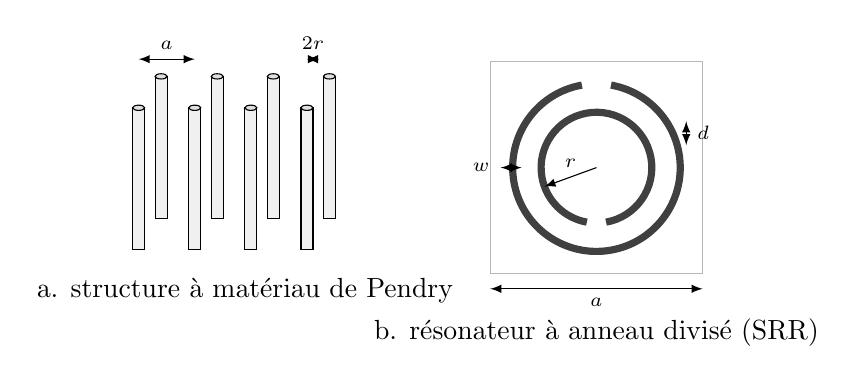
\begin{tikzpicture}[>=latex,scale=0.95]
    % --- (a) Pendry thin-wire medium
    \begin{scope}
      \foreach \i in {0,1,2,3} {
        \foreach \k in {0,1} {
          \pgfmathsetmacro{\xx}{\i*0.75 + \k*0.30}
          \pgfmathsetmacro{\yy}{\k*0.42}
          \draw[fill=gray!12] (\xx,\yy) rectangle (\xx+0.16,\yy+1.9);
          \draw[fill=gray!25] (\xx+0.08,\yy+1.9) ellipse (0.08 and 0.035);
        }
      }
      \draw[<->] (0.08,2.55) -- (0.83,2.55) node[midway,above]{\scriptsize $a$};
      \draw[<->] (2.33,2.55) -- (2.49,2.55) node[midway,above]{\scriptsize $2r$};
      \node at (1.5,-0.55) {a. structure à matériau de Pendry};
    \end{scope}
    % --- (b) circular split-ring resonator
    \begin{scope}[xshift=6.2cm,yshift=1.1cm]
      \draw[gray!55] (-1.42,-1.42) rectangle (1.42,1.42);
      \draw[line width=2.6pt,black!75] (100:1.12) arc (100:440:1.12);
      \draw[line width=2.6pt,black!75] (-80:0.74) arc (-80:260:0.74);
      \draw[<->] (-1.42,-1.62) -- (1.42,-1.62) node[midway,below]{\scriptsize $a$};
      \draw[->] (0,0) -- (200:0.74) node[midway,above]{\scriptsize $r$};
      \draw[<->] (1.2,0.30) -- (1.2,0.62);
      \node[right] at (1.22,0.46) {\scriptsize $d$};
      \draw[<->] (-1.28,0.0) -- (-1.00,0.0);
      \node[left] at (-1.30,0.0) {\scriptsize $w$};
      \node at (0,-2.2) {b. résonateur à anneau divisé (SRR)};
    \end{scope}
  \end{tikzpicture}
  \caption*{\small The two canonical cellules unitaires.
  The wire array gives $\varepsilon_{\mathit{eff}} < 0$ below the plasma
  pulsation; the résonateur à anneau divisé gives $\mu_{\mathit{eff}} < 0$ near
  its resonance.
  $a$ is the cell period, $r$ the inner-ring radius, $d$ the gap between rings,
  $w$ the ring width.}
\end{figure}

La structure tridimensionnelle proposée par Hudlicka est un autre exemple de
structure à permittivité négative à fils. Un treillis de fils connectés à
l'infini forme un élément \emph{triplet}. En utilisant l'approche du milieu
effectif, l'atténuation et les constantes de phase des modes qui se propagent
dans le milieu à triple fil ont été calculées à la fois au-dessous et au-dessus
de la fréquence du plasma. On a découvert que l'onde se propage en dessous de la
fréquence du plasma le long de \emph{toutes} les directions spatiales avec le
même facteur d'atténuation. Ainsi, la triple structure est caractérisée par
l'isotropie par rapport à la direction des ondes électromagnétiques --- which
the planar wire matrix is not.

\subsubsection{Perméabilité négative}

\begin{definition}[Résonateur à anneau divisé (\textit{split-ring resonator}, SRR)]
  La première structure à perméabilité négative, la plus utilisée, est le
  \textbf{résonateur à anneau divisé} (SRR). Les SRR peuvent être à la fois
  géométriquement ronds et carrés et sont caractérisés comme étant une
  structure \emph{résonante} hautement conductrice dans laquelle la capacité
  entre les deux anneaux équilibre l'inductance.
\end{definition}

Un champ magnétique variable dans le temps appliqué perpendiculairement à la
surface des anneaux induit des courants qui produisent le champ magnétique
secondaire. En fonction des propriétés de résonance de la structure, il peut
soit s'opposer au champ incident, soit le renforcer, which results in a
perméabilité effective $\mu_{\mathit{eff}}$ that is positive or negative.

\begin{prop}[Perméabilité effective d'un résonateur circulaire à double anneau fendu]
  Pour un résonateur circulaire, dans le vide, à double anneau fendu (on
  suppose une épaisseur négligeable) :
  \[
    \mu_{\mathit{eff}} = 1 -
      \frac{\pi r^2 / a}
           {1 - \dfrac{3d}{\pi^2\mu_0\varepsilon_0\varepsilon_r^{\,3}}
              + j\dfrac{2\sigma}{\omega\, r\mu_0}} ,
  \]
  où $a$ est la longueur unitaire de la cellule, $d$ est l'intervalle entre les
  anneaux, $r$ est le rayon de l'anneau intérieur et $\sigma$ est la
  conductivité électrique du métal formant l'anneau.
\end{prop}

\begin{remark}
  The formula above is the approximate expression of the perméabilité
  effective, and the narrow frequency band of the first drawback below is the
  one where $\mu_{\mathit{eff}} < 0$ --- that is the property being engineered.
  The secondary magnetic field likewise acts on the perméabilité, not on the
  permittivité: the quantity is $\mu$, never $\varepsilon$, and $\mu$ is the
  relevant quantity throughout the discussion of the SRR.
\end{remark}

\begin{conclusion}[Limits of the first SRRs]
  Les principaux inconvénients des premiers métamatériaux basés sur des
  résonateurs circulaires ou rectangulaires sont
  \begin{subpart}
    \item une bande de fréquence \emph{étroite}, over which the effect exists;
    \item des niveaux élevés de conductivité électrique, required of the metal;
    \item a strong dependence on l'incidence de l'onde éclairant la structure
      --- l'effet de perméabilité négative est observé sous incidence normale ou
      proche de la normale, ce qui réduit fortement le champ d'utilisation.
  \end{subpart}
  Les travaux actuels sont souvent liés à l'augmentation de la bande de
  fréquence ainsi qu'à une incidence d'ondes plus large. Diverses structures ont
  été élaborées sur différentes topologies (2D et 3D) modifiées pour répondre
  aux problèmes --- nested rings, rings loaded with capacitive stubs, tilted
  rings.
\end{conclusion}

\begin{remark}[What made the field famous]
  Ce qui a réellement attiré l'attention sur ces matériaux atypiques a été la
  proposition par J. Pendry de la possibilité de réaliser une
  \textbf{superlentille} (\textit{superlens}) dont la résolution ne serait plus
  limitée par les lois classiques de l'optique. En 2006, J. Pendry et
  U. Leonhardt proposaient la réalisation d'une \textbf{cape d'invisibilité}
  (\textit{invisibility cloak}) utilisant des métamatériaux. Le principe semble
  simple : on utilise un métamatériau dans lequel on fait entrer la lumière, qui
  contourne alors le centre pour reformer l'image initiale intacte de l'autre
  côté. On a alors l'illusion qu'il n'y a rien à l'intérieur du milieu. En
  l'occurrence, le métamatériau n'est pas une cape mais une \emph{sphère} qui
  est utilisée puisqu'elle doit être capable de couvrir tous les angles. Elle
  sera composée de résonateurs disposés sur des cercles concentriques. Ces
  différentes couches se distinguent par leur nombre de charges électriques
  puisque ce sont elles qui vont permettre de guider la lumière à l'intérieur du
  milieu. The demonstration is a cape d'invisibilité hyperfréquence réalisée au
  C2N (ex IEF) à Orsay (équipe André de Lustrac) : une sphère d'invisibilité
  capable de rendre invisible un cylindre d'une vingtaine de centimètres de
  diamètre.
\end{remark}

\subsection{Les métamatériaux dans les systèmes micro-ondes}

Les propriétés électrophysiques particulières des structures artificielles
composites permettent de les utiliser avec succès dans le domaine des
hyperfréquences. La plupart des métamatériaux, tels que les structures à
permittivité, perméabilité ou les 2 négatives sont activement mis en œuvre dans
les guides d'ondes, les résonateurs, les diviseurs de puissance, les
absorbeurs, filtres, coupleurs, isolateurs, antennes et leurs éléments
constructifs. On peut concevoir un guide d'ondes multibande, des réseaux et des
systèmes basés sur les métamatériaux, des composants à bande passante
améliorée, amplificateurs distribués, résonateurs d'ordre zéro, filtres
hyperfréquences avancés, etc.

\subsubsection{Les lignes de propagation}

Les milieux métamatériaux combinés --- negative in permittivité \emph{and} in
perméabilité --- ont trouvé une place dans les systèmes hyperfréquences. On a
découvert que les propriétés électromagnétiques non conventionnelles des
métamatériaux sont observées lorsqu'un matériau est associé avec un autre
matériau ayant au moins une constante matérielle effective de \emph{signe
opposé}.\\

Certaines propriétés sont utilisées sur les lignes de propagation telles que les
guides d'ondes à faces parallèles : en associant différentes couches, il est
possible d'obtenir un mode de propagation TEM avec les propriétés physiques
associées identiques à celles que l'on rencontre en espace libre.\\

Dans les lignes sur substrat, les utilisations de ces types de matériau sont
recherchées aussi, and the sought property is usually phase control. Un exemple
concerne les \textbf{coupleurs} (\textit{couplers}) : un coupleur utilisant une
\textbf{ligne de transmission « main gauche »} (\textit{left-handed line}, LH).

\begin{example}[Coupleur « main gauche »]
  L'ajout d'une structure dite à « main gauche » permet de contrôler la phase
  en sortie de coupleur. On peut obtenir ainsi deux sorties \emph{en phase} sans
  compensation de longueur sur des bandes de fréquence \emph{multiples}. En
  remplaçant les lignes de transmission conventionnelles dans les coupleurs par
  des structures LH, on a fabriqué un coupleur de branche à double bande de
  fréquence : en ajustant la phase en sortie de la ligne de transmission LH, le
  coupleur peut fonctionner à la fréquence fondamentale \emph{et} la première
  harmonique sans changer de structure.
\end{example}

Les coupleurs directionnels basés sur des lignes de transmission à métamatériau
présentent ainsi un couplage amélioré et une gamme de fréquences de
fonctionnement étendue en ayant des dimensions plus compactes par rapport aux
coupleurs conventionnels. Le phénomène de compensation de phase is
characteristic of \textbf{CRLH} (composite right/left-handed) structures. Plus
généralement l'exploitation de ces structures permet d'obtenir des déphaseurs à
large bande avec une erreur de phase faible, des filtres passe-bas et passe-haut
compacts à faibles pertes basés sur l'utilisation de la résonance de la
structure. On y assure de faibles pertes dans la bande et des pertes très
élevées en dehors de la bande tout en conservant une compacité impossible à
atteindre avec une structure traditionnelle.

\subsubsection{Les absorbeurs électromagnétiques micro-ondes}

Une branche particulière des applications est celle des \textbf{absorbeurs
électromagnétiques} (\textit{electromagnetic absorbers}) pour les bandes
hyperfréquences et térahertz. Ils sont constitués d'une couche de métamatériaux et
d'une plaque métallique séparée par un diélectrique; les résonateurs de base et
les dérivés sont largement utilisés comme éléments métamatériaux des absorbeurs
hyperfréquences.

\begin{conclusion}
  Les principaux avantages de ces absorbeurs sont la compacité et la facilité de
  fabrication avec une indépendance vis-à-vis de la polarisation dans une large
  bande de fréquences. Un facteur d'absorption élevé pour de larges angles
  d'incidence et la possibilité de réglage dynamique ont été obtenus.
  L'objectif principal de ces études est de concevoir des absorbeurs
  métamatériaux \emph{parfaits} qui fournissent un facteur d'absorption égal à
  l'unité dans une large gamme d'angles d'incidence et de fréquences. Des
  dispositifs capables d'absorber l'énergie électromagnétique en certains points
  et la transférer en chaleur ont été développés.
\end{conclusion}

Il est possible aussi d'accorder la fréquence de fonctionnement pour les
utiliser comme capteurs sensibles au spectre, notamment dans les
micro-bolomètres, mais l'application principale demeure la réduction de la
\textbf{surface équivalente radar} (\textit{radar cross-section}, SER; RCS in
English) d'un objet fortement réflecteur, comme dans les applications
militaires mais aussi satellites, en minimisant le volume et le poids de cette
structure additionnelle.

\subsubsection{Les antennes}

Dans le cadre de la conception d'antennes, les applications les plus répandues
se focalisent sur les antennes imprimées miniaturisées. Les caractéristiques
d'une antenne sont liées à ses dimensions, aussi réduire la taille d'une
antenne ne doit pas ou peu dégrader les performances nominales. L'une des
approches les plus efficaces pour améliorer le comportement des antennes
\emph{électriquement petites} est de couvrir le ou les éléments rayonnants par
un radom (capot de couverture) à métamatériau dont l'impédance équivalente est
adaptée avec l'espace environnant: for example a monopôle over a plan de masse,
covered by a hemispherical ENG radom of inner radius $r_2$ and outer radius
$r_1$.

\begin{conclusion}[What the radom buys]
  On peut donc réaliser des antennes à haut rendement avec un facteur de
  qualité supérieur en repoussant la limite fondamentale liée à la taille
  physique de l'antenne. Afin de compenser la puissance réactive, on utilise des
  matériaux à permittivité négative (ENG) à forte auto-inductance. En outre,
  l'épaisseur de la couche de métamatériau peut être inférieure au centième de
  la longueur d'onde, ce qui permet d'éviter toute atténuation notable dans ce
  type de système. L'utilisation de matériaux DNG permet d'améliorer la
  conception en réduisant davantage la taille physique et les coûts en
  compensant la puissance rayonnée.
\end{conclusion}

Métamatériaux also go into substrates: l'application dans des \emph{substrats}
pour antennes miniaturisées imprimées permet de réduire la taille des éléments
rayonnants conventionnels, d'augmenter la largeur de bande de l'antenne et
d'améliorer l'efficacité de rayonnement. La structure du substrat est homogène
comme d'habitude et est composée de SRR, d'anneaux chiraux ou de
métasolénoïdes ou en comporte plusieurs types dans une même structure. Il
devient intéressant d'employer les technologies de lignes d'alimentation
« main gauche » pour des antennes réseaux afin de réduire la taille globale de
l'antenne réalisée et de supprimer les interférences des éléments rayonnants
adjacents.\\

Les métamatériaux ont aussi un rôle crucial pour les antennes à réflecteur. On
peut ainsi plaquer l'antenne sur son réflecteur annulant ainsi l'espace entre
les 2, ce qui en réduit le volume global ou, for a mast-mounted antenne, la
prise au vent. À Telecom Paris, une activité reconnue de recherches concerne la
réduction de dimensions des absorbeurs à métamatériau ainsi que celle des
antennes exploitant un \emph{réflecteur magnétique} à métamatériau.

\begin{example}[Réflexion sur un conducteur métallique et sur un conducteur magnétique]
  On place une source d'ondes planes à une hauteur $h < \lambda$ au-dessus
  d'un réflecteur infini ; le réflecteur est modélisé par un facteur de
  réflexion scalaire $\Gamma$, and the quantity sought is le vecteur de
  Poynting résultant de la superposition des ondes directes et réfléchies.\\

  A \emph{metallic} réflecteur has $\Gamma = -1$: the reflected field arrives
  back at the source with a phase $2kh + \pi$, so the two waves add
  constructively in the axis only when $2kh = \pi$, that is
  \[ h = \frac{\lambda}{4}. \]
  The réflecteur must stand a quarter of a longueur d'onde away, which sets the
  usable band and makes the assembly thick.\\

  Un \textbf{conducteur magnétique artificiel} (\textit{artificial magnetic
  conductor}) --- a métamatériau, in contrast --- se caractérise par un
  facteur de réflexion complexe égal à $+1$, ce qui correspond à une
  \emph{impédance de surface infinie}. The reflected field returns in phase for
  $h \to 0$, so the réflecteur can be brought right up against the radiating
  element. That is the advantage of this solution. Deux exemples de plan
  réflecteur magnétique ou métamatériaux (pavage cartésien et concentrique)
  placés en dessous d'une antenne large bande de type spirale d'Archimède
  (antenne bidirectionnelle à polarisation circulaire) : l'objectif est
  d'obtenir une antenne unidirectionnelle (avec un gain augmenté) tout en
  restant mince (ce qu'il est impossible d'obtenir avec un réflecteur
  métallique).
\end{example}

\begin{remark}[References]
  Buriak \textit{et al.}, ``Metamaterials: Theory, Classification and
  Application Strategies'', \textit{J. Nano- Electron. Phys.} \textbf{8}(4)
  (2016), for the survey; Pendry, Holden, Robbins and Stewart, \textit{IEEE
  Trans.\ MTT} (1998), for the medium of fils métalliques minces; Hudlicka,
  Machac and Nefedov,
  \textit{PIER} \textbf{65} (2006), for the 3D triplet lattice; Eleftheriades
  and Balmain, \textit{Negative-refraction Metamaterials} (IEEE--Wiley, 2005),
  for the general theory; and Djoma \textit{et al.}, ``Maximal Bandwidth of an
  Archimedean Spiral Antenna Above a Reflector'', \textit{IEEE AWPL}
  \textbf{13} (2014), for the spiral antenne over a réflecteur of the example
  above.
\end{remark}
